
\chapter{Applications of Deep Learning in Visual Recognition of Wheat Diseases}

\section{Introduction}

The spread of wheat diseases poses serious threats to agricultural productivity and food security. Early and accurate detection is essential for timely intervention and disease management. In this context, deep learning has emerged as a powerful approach to support smart agriculture by enabling automated, data-driven solutions.

This chapter focuses on the application of deep learning techniques to visual data, particularly images captured in the field. It highlights three key computer vision tasks used in precision agriculture: image classification, image segmentation, and object detection. These tasks allow machines to recognize disease types, locate affected areas on plant surfaces, and detect objects such as crops or weeds in complex environments. The chapter begins with the fundamentals of deep neural networks and proceeds to how they are used for agricultural image analysis. It also introduces practical techniques like transfer learning and fine-tuning, which help adapt models to specific agricultural datasets.

% \section{Distinctions between deep learning and machine learning}
% \gls{abb:dl} is a subset of \gls{abb:ml} that uses \gls{abb:dnn}s to automatically learn complex patterns from large, unstructured data like images, text, and audio. Unlike traditional \gls{abb:ml}, which requires manual feature extraction and works best with smaller, structured datasets, \gls{abb:dl} eliminates this need and can handle large datasets with significant computational power, often using \gls{abb:gpu}s. While \gls{abb:ml} is suitable for tasks like predictive analytics, \gls{abb:dl} excels in applications such as image recognition, speech processing, and natural language understanding.\parencite{AlvarezVanhard2021}.


\section{Deep learning fundamentals}
In this section, we introduce the core principles of \gls{abb:dl}, focusing on \gls{abb:dnn} and their role in learning complex patterns from data. We explore the structure and components of neural networks, the learning process, optimization techniques, and model evaluation methods. Additionally, we highlight regularization strategies to prevent overfitting.

\subsection{Deep neural network basics (DNN)}
Neural networks form the backbone of deep learning, enabling machines to learn patterns and make predictions from data. Inspired by the structure of the human brain, these networks consist of interconnected layers of artificial neurons that hierarchically process information.

\subsubsection{Definition of DNN}

Before defining deep neural networks, we first need to understand two essential components: 
\begin{itemize}
    \item \textbf{Artificial neuron}: An artificial neuron is the basic building block of artificial neural networks, designed based on the structure and functionality of biological neurons. It receives weighted inputs, processes them through a transfer function, and outputs the result. The artificial neuron model simplifies the biological process where information is received through dendrites, processed in the soma, and transmitted via the axon, as shown in Figure~\ref{fig:figure01} \parencite{krenker2011introduction}.
    
    \item \textbf{Layer}: A layer in a neural network is a set of neurons that perform a specific operation on the data \parencite{bengio2017deep}.
\end{itemize}

\begin{figure}[H] % 'H' needs \usepackage{float}
    \centering
    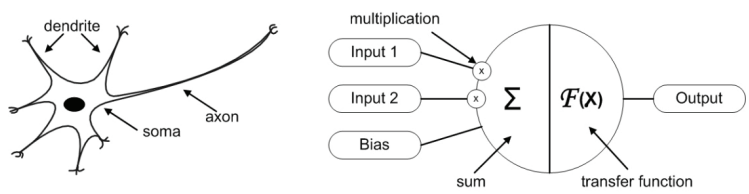
\includegraphics[width=0.8\textwidth]{chapters/chapter02/images/Figure01.png}
    \caption{Biological Neuron Structure and Its Mathematical Model Representation \parencite{krenker2011introduction}.}
    \label{fig:figure01}
\end{figure}


By combining multiple layers of interconnected artificial neurons, we arrive at the concept of a Deep Neural Network (DNN). A DNN is a neural network that contains multiple hidden layers between the input and output layers. These additional layers enable the network to learn complex patterns and high-level features from data. Each layer transforms its input into a more abstract representation, improving the network’s ability to recognize intricate structures and relationships \parencite{li2021water}.
\subsubsection{Structure of DNN}
A neural network (Figure~\ref{fig:figure03}) consists of three main layers \parencite{ren2023review}:

\noindent
\textbf{The input layer:} Represents the features of the input data, such as pixel values in an image, denoted as a vector 
\[
X = [x_1, x_2, \dots, x_n].
\]

\noindent
\textbf{The hidden layers:} Process this input using weighted connections and biases, computed as:
\[
z = W \cdot X + b_z \tag{1}
\]
\[
F(z) = a \tag{2}
\]
where:
\begin{itemize}
    \item $W$ is the weight matrix,
    \item $b$ is the bias vector,
    \item $z$ is the pre-activation value,
    \item $F(z)$ is the activation function applied to $z$.
\end{itemize}

Each neuron in the hidden layers applies an activation function to capture complex patterns.

\noindent
\textbf{The output layer:} Generates the network's prediction, with the number of neurons corresponding to the specific task, such as one neuron for binary classification or multiple neurons for multiclass classification.



\begin{figure}[H] % 'H' needs \usepackage{float}
    \centering
    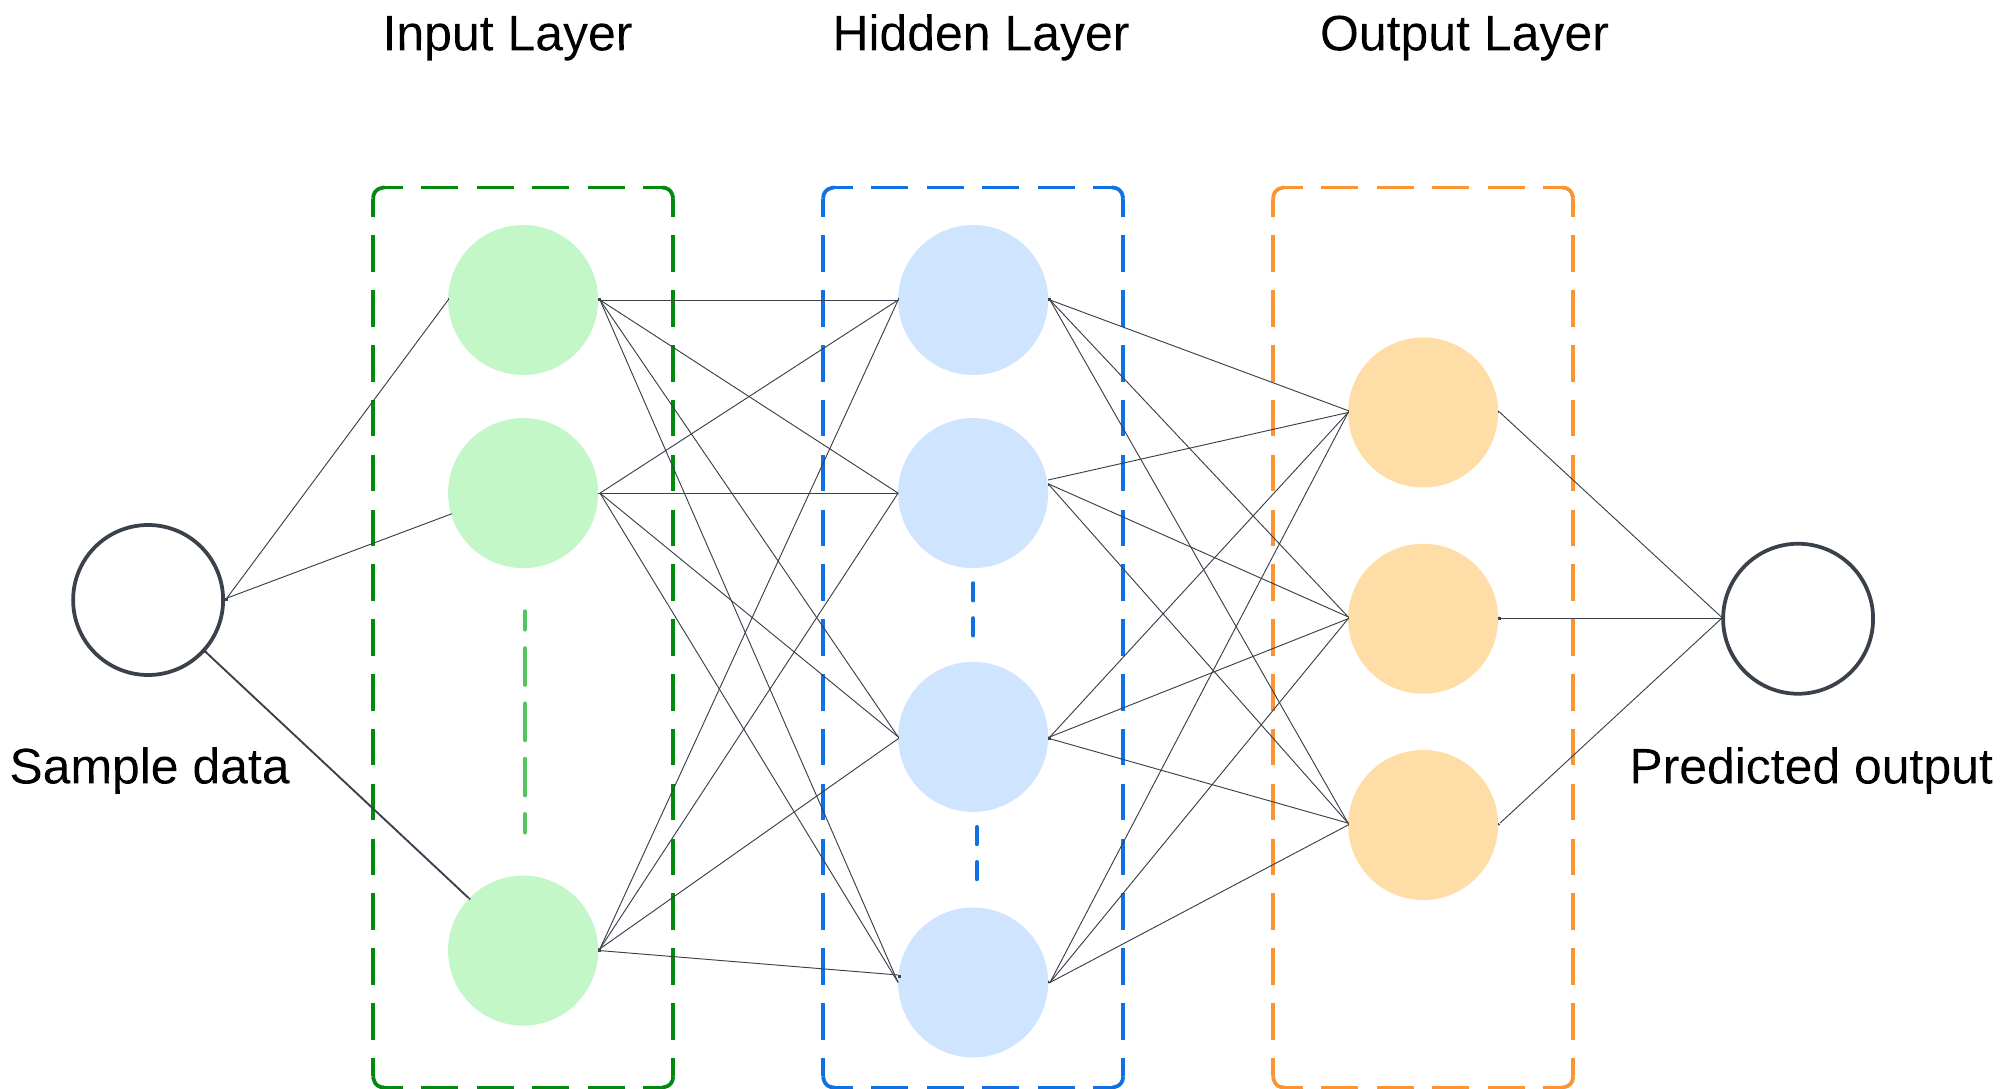
\includegraphics[width=0.8\textwidth]{chapters/chapter02/images/DNN.png}
    \caption{The structure of the DNN \cite{ren2023review}.}
    \label{fig:figure03}
\end{figure}


% \begin{figure}[H] % 'H' needs \usepackage{float}
%     \centering
%     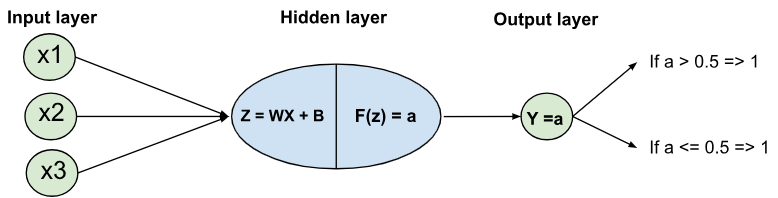
\includegraphics[width=0.6\textwidth]{chapters/chapter1/images/Figure02.png}
%     \caption{The structure of a Neural Network in the binary classification task.}
%     \label{fig:figure02}
% \end{figure}

\subsubsection{Activation functions (AF)}
An \gls{abb:af} is a mathematical function applied to a neuron's output in a neural network to introduce non-linearity. Without an activation function, a neural network with multiple layers would behave like a single-layer perceptron, limiting its ability to model complex relationships \parencite{dubey2022activation}. Activation functions decide whether a neuron should be activated based on its input. Here are some used activation functions in \gls{abb:dnn} models \parencite{dubey2022activation}:

\begin{itemize}
    \item \textbf{Sigmoid function}: Commonly used in binary classification problems, especially in the output layer of models predicting probabilities. It maps input values to a range between 0 and 1, making it suitable for representing probabilities, as shown in equation~\ref{eq:sigmoid}.
    \begin{equation}
        \text{Sigmoid}(x) = \frac{1}{1 + e^{-x}}
        \label{eq:sigmoid}
    \end{equation}
    
    \item \textbf{Tanh (Hyperbolic tangent)}: Often used in hidden layers of neural networks. It outputs values centered around zero, helping reduce bias during optimization. Its formulation is given in equation~\ref{eq:tanh}.
    \begin{equation}
        \tanh(x) = \frac{e^{x} - e^{-x}}{e^{x} + e^{-x}}
        \label{eq:tanh}
    \end{equation}

    \item \textbf{ReLU (Rectified linear unit)}: Widely used in hidden layers due to its simplicity and effectiveness in handling the vanishing gradient problem. It outputs zero for negative inputs and the input itself for positive values, as defined in equation~\ref{eq:relu}.
    \begin{equation}
        \text{ReLU}(x) = \max(0, x)
        \label{eq:relu}
    \end{equation}

    \item \textbf{Softmax function}: Used in the output layer for multi-class classification. It converts a vector of values into a probability distribution, as illustrated in equation~\ref{eq:softmax}.
    \begin{equation}
        \text{Softmax}(x_i) = \frac{e^{x_i}}{\sum_j e^{x_j}}
        \label{eq:softmax}
    \end{equation}
    where $x_i$ is the current element and the denominator sums over all elements $x_j$ in the vector.
\end{itemize}

% \subsubsection{Activation functions}
% An activation function is a mathematical function applied to a neuron's output in a neural network to introduce non-linearity. Without an activation function, a neural network with multiple layers would behave like a single-layer perceptron, limiting its ability to model complex relationships \parencite{dubey2022activation}. Activation functions decide whether a neuron should be activated based on its input. Table \ref{tab:activation-functions} summarizes the most commonly used activation functions, their formulas, ranges, and typical use cases in deep neural networks.

% \begin{table}[htbp]
%     \caption{Common Activation Functions in Deep Learning \parencite{dubey2022activation}}
%     \centering
%     \resizebox{\textwidth}{!}{%
%     \begin{tabular}{|p{3cm}|p{4.5cm}|p{3cm}|p{3.5cm}|}
%     \hline
%     \textbf{Activation Function} & \textbf{Formula} & \textbf{Range} & \textbf{Usage} \\
%     \hline
%     Sigmoid                      & $\text{Sigmoid}(x) = \frac{1}{1+e^{-x}}$         & [0, 1]               & Commonly used in binary classification problems, especially in the output layer of models predicting probabilities. \\
%     \hline
%     Tanh (Hyperbolic Tangent)     & $\tanh(x) = \frac{e^{x} - e^{-x}}{e^{x} + e^{-x}}$ & [-1, 1] & Often used in hidden layers of neural networks, as it outputs values centered around zero, which helps in reducing bias during optimization. \\
%     \hline
%     ReLU (Rectified Linear Unit)  & $\relu(x) =\text{max}(0, x)$            & [0, $\infty$)        & Widely used in hidden layers of deep neural networks due to its simplicity and effectiveness in handling the vanishing gradient problem. \\
%     \hline
%     Softmax & $\text{Softmax}(x_i) = \frac{e^{x_i}}{\sum_j e^{x_j}}$, where $x_i$: current element, $x_j$: all elements in the vector. & (0, 1) (outputs sum to 1) & Used in the output layer for multi-class classification. \\
%     \hline

%     \end{tabular}%
%     }
%     \label{tab:activation-functions}
% \end{table}


    
\subsection{Learning process in deep neural networks}

In the information processing flow within an artificial neuron, several elements, known as parameters, are learned from the training data. These parameters include \parencite{Kelleher2019}:
\begin{itemize}
    \item \textbf{Weights}: Weights control the amount of each input feature that passes through the neuron. They represent the coefficients of the connections between neurons in the layers of a neural network. Weights are essential for determining the influence of each input on the output.
    
    \item \textbf{Biases}: Biases are values added to the outputs of the neurons before applying the activation function. They allow the network to shift the activation function, providing more flexibility to the model.
\end{itemize}

The learning process in neural networks involves training the model to map input data to desired outputs. This is achieved through the mechanisms of forward propagation and backward propagation, along with optimization techniques that refine the network's parameters (weights and biases) to minimize the error \parencite{Kelleher2019}:
\begin{itemize}
    \item \textbf{Forward Propagation}: In forward propagation, the input data passes through the network layer by layer. Each neuron in a layer performs a weighted sum of its inputs, applies an activation function, and passes the result to the next layer. The process continues until the output layer is reached and a prediction is made.
    
    \item \textbf{Backward Propagation}: Backward propagation (or backpropagation) is used to update the network's weights. After calculating the error (the difference between the predicted and actual output), the error is propagated back through the network. The weights are adjusted based on the gradient of the error with respect to each weight, using optimization algorithms like gradient descent.
\end{itemize}

% Figure \ref{fig:figure03} below provides a visual representation of the learning process in a neural network, illustrating the flow of information from the input layer through multiple hidden layers to the output layer.


% \begin{figure}[H] % 'H' needs \usepackage{float}
%     \centering
%     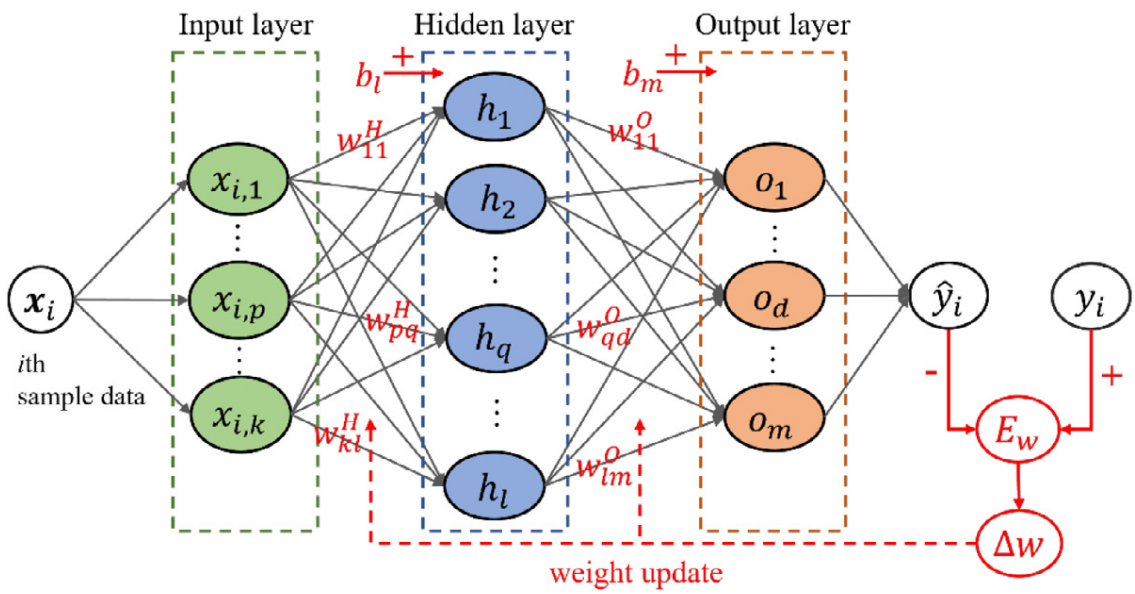
\includegraphics[width=0.6\textwidth]{chapters/chapter02/images/Figure03.png}
%     \caption{The structure of the DNN \cite{ren2023review}.}
%     \label{fig:figure03}
% \end{figure}



\subsection{Model training concepts}

Effective model training ensures that neural networks learn patterns in data while minimizing errors. This section highlights essential components of the training process.

\subsubsection{Loss Functions} 
Loss functions quantify the error between predicted and actual values, guiding weight updates during optimization \parencite{alzubaidi2021review}. Common loss functions include:
\begin{itemize}
    \item \textbf{Cross-Entropy Loss}: Used for classification tasks to measure the divergence between predicted probabilities and true labels.
    \item \textbf{Mean Squared Error (MSE)}: Applied in regression, computing the average squared difference between predicted and actual values.
\end{itemize}

\subsubsection{Overfitting prevention}
Overfitting occurs when a model learns noise from training data, reducing generalization to unseen data. Common techniques to mitigate overfitting include:
\begin{itemize}
    \item \textbf{Dropout}: Randomly deactivate neurons during training to enhance robustness.
    \item \textbf{Data Augmentation}: Transform training samples (e.g., rotation, scaling) to increase dataset diversity.
\end{itemize}

\subsubsection{Batch normalization}
Batch Normalization normalizes layer outputs to follow a unit Gaussian distribution, a normal distribution with a mean of 0 and a standard deviation of 1, which keeps values in a consistent range and stabilizes learning. This helps stabilize and speed up neural network training by reducing internal covariance shift, which is caused by changing activation distributions during training, especially with diverse data sources. Key benefits include preventing vanishing gradients, improving weight initialization, speeding up convergence, and reducing sensitivity to hyperparameters \parencite{alzubaidi2021review}.


\subsection{Optimization methods and strategies}
Optimization techniques in deep learning are methods used to minimize the loss function during training, improving the model’s accuracy. These techniques adjust the model's weights and biases iteratively to find the optimal set of parameters that reduces the error between predicted and actual values \parencite{alzubaidi2021review}.

Different optimizers are used to update model weights efficiently:

\begin{itemize}
    \item \textbf{Stochastic Gradient Descent (SGD):} Updates weights based on a small subset (batch) of training data, improving computational efficiency.
    \item \textbf{Adam (Adaptive Moment Estimation):} Combines momentum and adaptive learning rates for faster and more stable convergence.
    \item \textbf{RMSprop:} Uses an adaptive learning rate to prevent oscillations and improve performance on non-stationary objectives.
\end{itemize}

% However, an important consideration in optimization is how to set the learning rate throughout training. While optimizers control how weights are updated, learning rate scheduling adjusts the learning rate over time to further optimize training.
% Different scheduling strategies can be used in conjunction with optimizers \parencite{zhao2019learningrate}:

% \begin{itemize}
%     \item \textbf{Step Decay:} Reduces the learning rate at fixed intervals, allowing for more stable training as the model reaches its optimal solution.
%     \item \textbf{Exponential Decay:} Gradually decreases the learning rate across epochs, promoting finer adjustments to the model parameters as the training progresses.
%     \item \textbf{Cyclic Learning Rates:} Alternates between a minimum and maximum learning rate, which helps the model escape local minima and enhances exploration of the parameter space.
% \end{itemize}

% By combining these scheduling strategies with optimization techniques, the training process can become more efficient and effective, leading to faster and more reliable convergence.






\subsection{Model evaluation and validation}

Once a model is trained, it is crucial to assess its performance and ensure that it generalizes well to unseen data. This process is known as \textbf{model evaluation and validation}. The primary goal is to measure how well the model performs and to identify any potential overfitting or underfitting issues.

To evaluate a model’s performance, several metrics can be used depending on the type of task (classification, regression, etc.) \parencite{ketkar2017deep}:
\begin{itemize}
    \item \textbf{Accuracy:} For classification tasks, accuracy measures the proportion of correct predictions out of all predictions made. However, accuracy alone can be misleading in imbalanced datasets.
    \item \textbf{Precision and Recall:} In imbalanced classification problems, precision (the proportion of true positive results among all positive predictions) and recall (the proportion of true positive results among all actual positives) are often used in conjunction to provide a clearer view of the model's performance.
    \item \textbf{F1-Score:} The harmonic mean of precision and recall; F1-score balances the two metrics and is especially useful when dealing with imbalanced datasets.
    \item \textbf{Mean Squared Error (MSE):} For regression tasks, MSE calculates the average of the squared differences between predicted and actual values. It penalizes large errors more significantly than smaller ones.
    \item \textbf{R-squared (R²):} For regression, this metric indicates how well the model explains the variability in the data, with a value closer to 1 suggesting a better fit.
\end{itemize}


% \section{Deep Learning Approaches}

% Deep learning encompasses a variety of learning paradigms that enable models to extract complex patterns from large volumes of data. These approaches differ based on the nature of the data, the availability of labels, and the interaction mechanisms with the environment. This section presents the four main categories of deep learning methods \parencite{alzubaidi2021review}:

% \begin{itemize}
%     \item \textbf{Deep Supervised Learning:} This approach involves training a neural network using a labeled dataset, where each input image (e.g., leaf with visible symptoms) is paired with its correct label (e.g., disease type). The model learns to minimize the error between its predictions and the true labels using backpropagation and optimization algorithms. Techniques include Convolutional Neural Networks (\gls{abb:cnn}s) for spatial feature extraction, Deep Neural Networks (DNNs), and Recurrent Neural Networks (RNNs) like LSTMs and GRUs when dealing with sequential data.
    
%     \item \textbf{Deep Semi‐Supervised Learning:} Semi-supervised learning combines a small labeled dataset with a larger pool of unlabeled data, which is common in agricultural settings where annotating plant diseases is costly and time-consuming. Methods like Generative Adversarial Networks (GANs) can generate synthetic labeled images, while RNNs, LSTMs, and Deep Reinforcement Learning (DRL) can help model complex data behavior.
    
%     \item \textbf{Deep Unsupervised Learning:} Unsupervised learning aims to extract meaningful patterns from unlabeled data, such as grouping similar plant images or identifying features without predefined classes. Popular methods include Autoencoders for dimensionality reduction, Restricted Boltzmann Machines, and clustering algorithms. These are useful in exploratory stages or feature extraction before applying a classifier.
    
%     \item \textbf{Deep Reinforcement Learning (DRL):} In DRL, models learn optimal actions through trial and error by interacting with an environment. This could include real-time monitoring systems in agriculture, like automated disease response tools or robotic weeders. Unlike supervised learning, DRL does not require labeled data but instead uses reward signals to adjust its strategy over time.
% \end{itemize}

\section{Core computer vision tasks in agriculture}

The most common and impactful computer vision tasks include image classification, image segmentation, and object detection. Each of these tasks plays a vital role in applications such as disease diagnosis, crop monitoring, yield estimation, and weed or pest detection. The following sections explore these tasks and their corresponding deep learning techniques in detail.
\subsection{Image classification}
Image classification is the task of assigning a label to an entire image based on its visual content. In deep learning, this is typically achieved using \gls{abb:cnn}s, which are designed to automatically learn hierarchical features from raw pixel data.

\subsubsection{Fundamentals of \gls{abb:cnn}s}
\gls{abb:cnn}s (Figure~\ref{fig:cnns_archi}) consist of multiple layers designed to process and learn spatial hierarchies from image data \parencite{alzubaidi2021review}. Their architecture typically includes:

% \begin{figure}[H] % 'H' needs \usepackage{float}
%         \centering
%         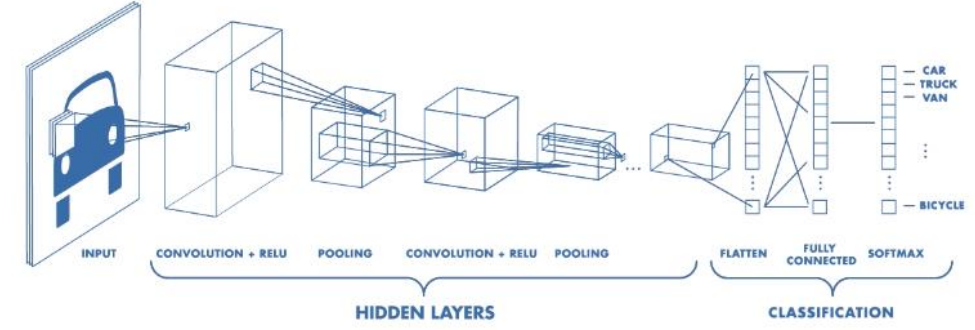
\includegraphics[width=0.9\textwidth]{chapters/chapter1/images/Figure04.png}
%         \caption{Architecture of \gls{abb:cnn} \cite{purwono2022understanding}.}
%         \label{fig:figure04}
%     \end{figure}


\begin{figure}[H] % 'H' needs \usepackage{float}
        \centering
        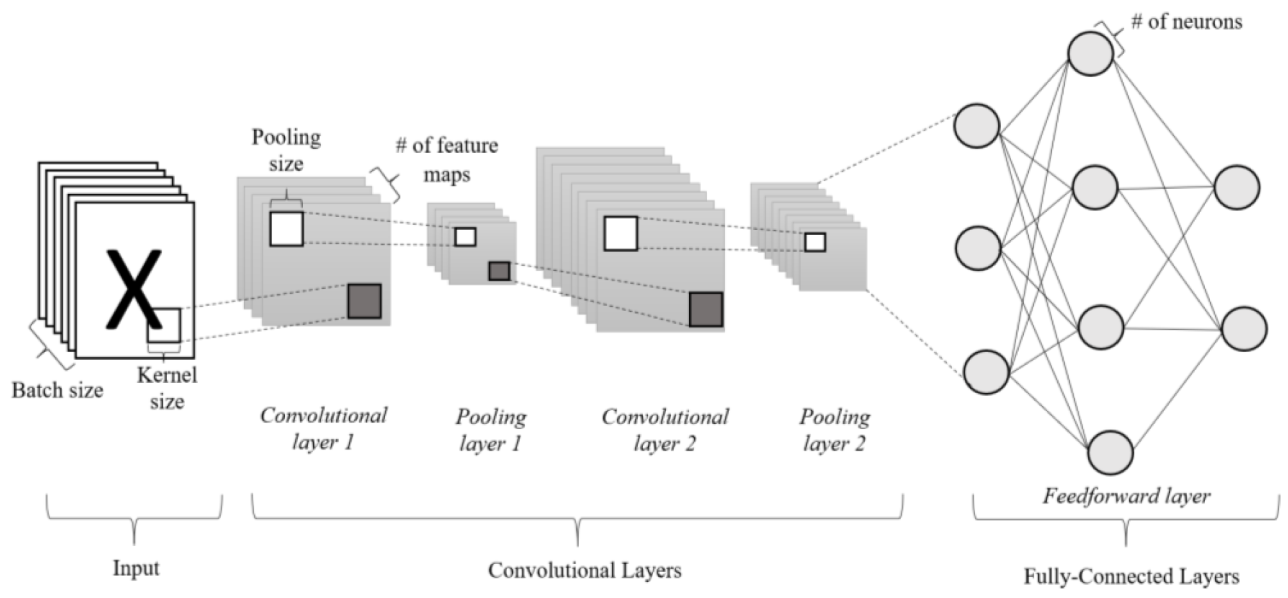
\includegraphics[width=0.9\textwidth]{chapters/chapter02/images/CNNarchitecture.png}
        \caption{Architecture of CNN \parencite{Ang2022Optimal}.}
        \label{fig:cnns_archi}
    \end{figure}

\begin{itemize}
    \item \textbf{Convolutional Layers:} Extract features using small filters (kernels) that detect edges, textures, and patterns. A kernel is a grid of values (weights) initialized randomly at the start of training and adjusted through learning to identify important features.
     
     
    \begin{itemize}
        \item \textbf{Input and Kernel Dimensions:} In a \gls{abb:cnn} layer, each input $x$ is structured in three dimensions: height, width, and depth. The depth corresponds to the number of channels (e.g., an \gls{abb:rgb} image has three channels). Similarly, the kernels are also three-dimensional, with spatial dimensions (height and width) and a depth matching the input channels. Each kernel has shared parameters, a set of weights and a bias. When applied to the input, these kernels generate a corresponding set of feature maps. These kernels establish local connections by interacting only with small regions of the input at a time, allowing the network to extract patterns such as edges and textures by computing dot products across these regions.
\item \textbf{Convolutional operation:} Mathematically, a 2D convolution operation between an input matrix $I$ and a kernel (or filter) $K$ is expressed as shown in equation~\ref{eq:convolution}:

        \begin{equation}
        S(i, j) = \sum_{m} \sum_{n} I(i + m, j + n) \cdot K(m, n)
        \label{eq:convolution}
        \end{equation}

        where $S(i, j)$ is the output feature map value at position $(i, j)$, $I$ is the input image, and $K$ is the kernel.

        The convolutional process involves sliding the kernel across the input image in both horizontal and vertical directions. At each location, the dot product between the kernel and the overlapping region of the input is computed, producing a scalar value that becomes part of the resulting feature map. As this process is repeated across the image, a full feature map is constructed, highlighting areas where the kernel detects specific patterns. Parameters such as stride (which controls how far the kernel moves at each step) and padding (which adds borders to the input to preserve edge information) affect the size and coverage of the output feature map. These concepts are illustrated in Figure~\ref{fig:figure05}.
     \end{itemize}   
    
     
    
    \begin{figure}[H] % 'H' needs \usepackage{float}
        \centering
        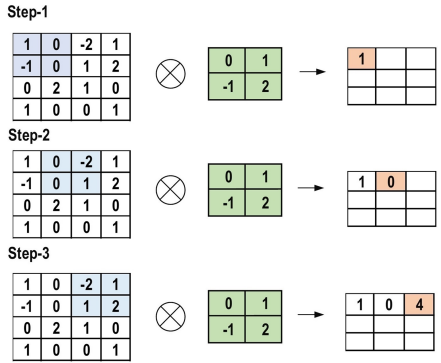
\includegraphics[width=0.6\textwidth]{chapters/chapter02/images/Figure05.png}
        \caption{The primary calculations executed at each step of the convolutional layer \parencite{alzubaidi2021review}.}
        \label{fig:figure05}
    \end{figure}

    \item \textbf{Pooling Layers:} Pooling layers are used to reduce the spatial dimensions of feature maps while preserving the most important information. This reduction helps lower the computational cost and minimizes the risk of overfitting by simplifying the data representation. The pooling operation works by sliding a small filter over the feature map and applying a summary function within each local region (Figure~\ref{fig:figure06}). Common types of pooling include:
    \begin{itemize}
        \item \textbf{Max Pooling:} Selects the maximum value in each region.
        \item \textbf{Average Pooling:} Calculates the average value of the region.
        \item \textbf{Global Average Pooling:} Computes the average across the entire feature map.
     \end{itemize}  
    
     \begin{figure}[H] % 'H' needs \usepackage{float}
        \centering
        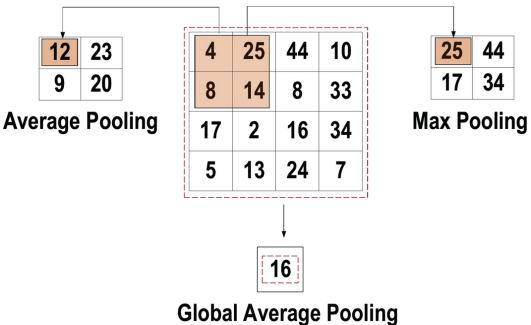
\includegraphics[width=0.6\textwidth]{chapters/chapter02/images/Figure06.png}
        \caption{Three types of pooling operations \parencite{alzubaidi2021review}.}
        \label{fig:figure06}
    \end{figure}
 
    % \item \textbf{Activation Functions:} Introduce non-linearity to help the network learn complex patterns. They must also be differentiable to enable backpropagation during training. \gls{abb:cnn}s commonly utilize the following activation functions: ReLU (Rectified Linear Unit), Sigmoid, Softmax, and Tanh.
    \item \textbf{Fully Connected Layers:} The Fully Connected (FC) layer is typically found at the end of a \gls{abb:cnn} architecture and serves as the classifier. In this layer, each neuron is connected to all neurons from the previous layer, following the fully connected approach. It operates similarly to a conventional \gls{abb:mlp} network, which is a type of feed-forward \gls{abb:ann}. The input to the FC layer is a vector created from the feature maps after flattening, which comes from the last pooling or convolutional layer. The output of the FC layer represents the final result of the classification task.
    
\end{itemize}

% Figure~\ref{fig:figure07} below illustrates the general structure of a \gls{abb:cnn}, highlighting its layers, which work together to extract and classify features from input images.

% \begin{figure}[H] % 'H' needs \usepackage{float}
%     \centering
%     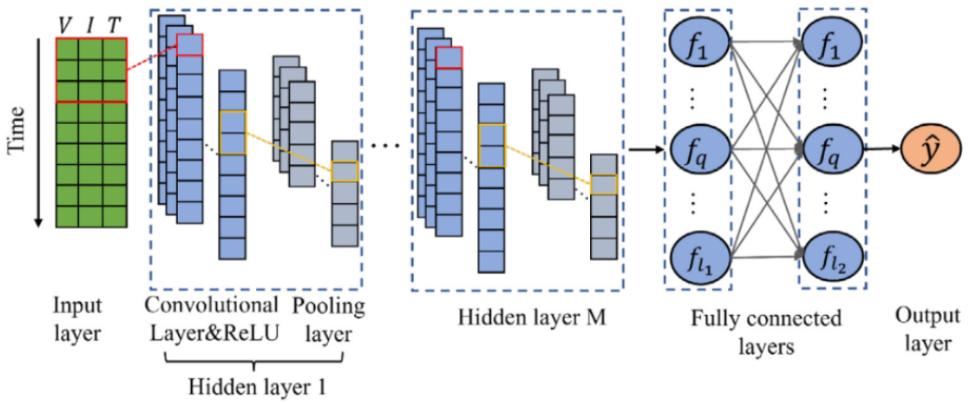
\includegraphics[width=0.9\textwidth]{chapters/chapter02/images/Figure07.png}
%     \caption{The structure of the \gls{abb:cnn} \parencite{crocioni2020li}.}
%     \label{fig:figure07}
% \end{figure}


\subsubsection{Convolutional Neural Network Architectures for Image Classification}

Over the past decade, various Convolutional Neural Network (CNN) architectures have been developed, each incorporating unique design principles to enhance accuracy, efficiency, and scalability. In image classification tasks particularly in plant disease detection the choice of architecture plays a crucial role, influenced by dataset size, complexity, and computational constraints.

Among these, lightweight and specialized models such as MobileNet, EfficientNet, and ShuffleNet have been designed to address speed, size, and energy limitations, making them ideal for mobile and edge device deployment. A comparative overview of both standard and lightweight CNN architectures, along with their key characteristics and potential use in smart agriculture, is provided in Appendix~\ref{app:annexA}.

\subsubsection{Transfer learning and pretrained models}
% In deep learning, training models from scratch often requires large labeled datasets and significant computational resources. Transfer learning offers a powerful alternative by leveraging models pre-trained on large benchmark datasets such as \textbf{ImageNet}. These pre-trained models capture rich and generalizable features in their initial layers, which can then be adapted to new, often smaller, target datasets with minimal additional training.
% This section explores the concept of transfer learning, introduces popular pre-trained \gls{abb:cnn} architectures relevant to agricultural applications, and outlines fine-tuning strategies suitable for small-scale plant datasets.

% \subsection{Concept of Transfer Learning}
Transfer learning is a machine learning technique where a model trained on one task is repurposed for a different but related task. In the context of deep learning, it typically involves taking a neural network pre-trained on a large dataset such as ImageNet, which contains over 14 million labeled images, and adapting it to a specific task that may lack sufficient labeled data.

To formalize this, consider a target learning task \( T_t \) based on a domain \( D_t \); transfer learning allows for assistance from a different domain \( D_s \) for the learning task \( T_s \). The goal of transfer learning is to improve the performance of the predictive function \( f_{T_t}(\cdot) \) for the task \( T_t \) by discovering and transferring latent knowledge from \( D_s \) and \( T_s \), where generally \( D_s = D_t \) and/or \( T_s = T_t \). Furthermore, it is often the case that the size of \( D_s \) is much larger than that of \( D_t \) \parencite{tan2018survey}.

% This process is illustrated in Figure~\ref{fig:figure14}, which demonstrates how knowledge from a source task and domain can be transferred to a target task with limited data.

% \begin{figure}[H] % 'H' needs \usepackage{float}
%     \centering
%     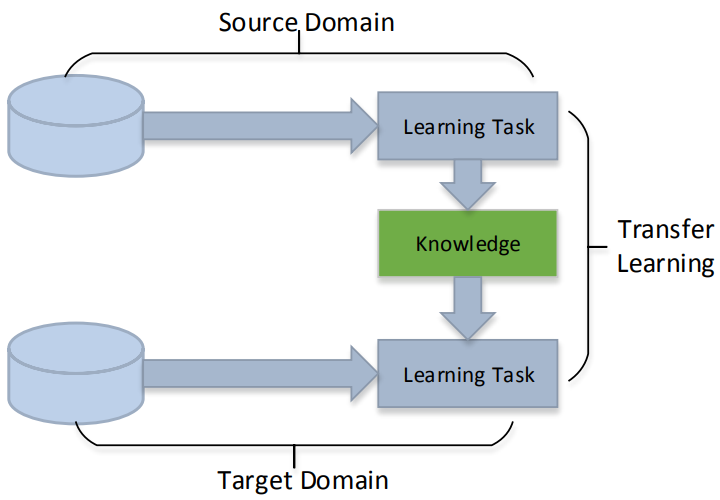
\includegraphics[width=0.5\textwidth]{chapters/chapter02/images/Figure14.png}
%     \caption{Learning process of transfer learning \parencite{tan2018survey}.}
%     \label{fig:figure14}
% \end{figure}
The two primary approaches to transfer learning are \parencite{tan2018survey}:

\begin{itemize}
    \item \textbf{Feature Extraction:} The pre-trained model is used as a fixed feature extractor. All convolutional layers are kept frozen, and only the final fully connected layer(s) are trained on the new dataset.
    \item \textbf{Fine-Tuning:} Some layers of the pretrained model are unfrozen and retrained on the new dataset. This allows the model to slightly adjust its learned features to better suit the new domain.
\end{itemize}

% This concept is illustrated in Figure~\ref{fig:figure15}, which demonstrates the integration of a custom \gls{abb:cnn} with transfer learning networks.

% \begin{figure}[H] % 'H' needs \usepackage{float}
%     \centering
%     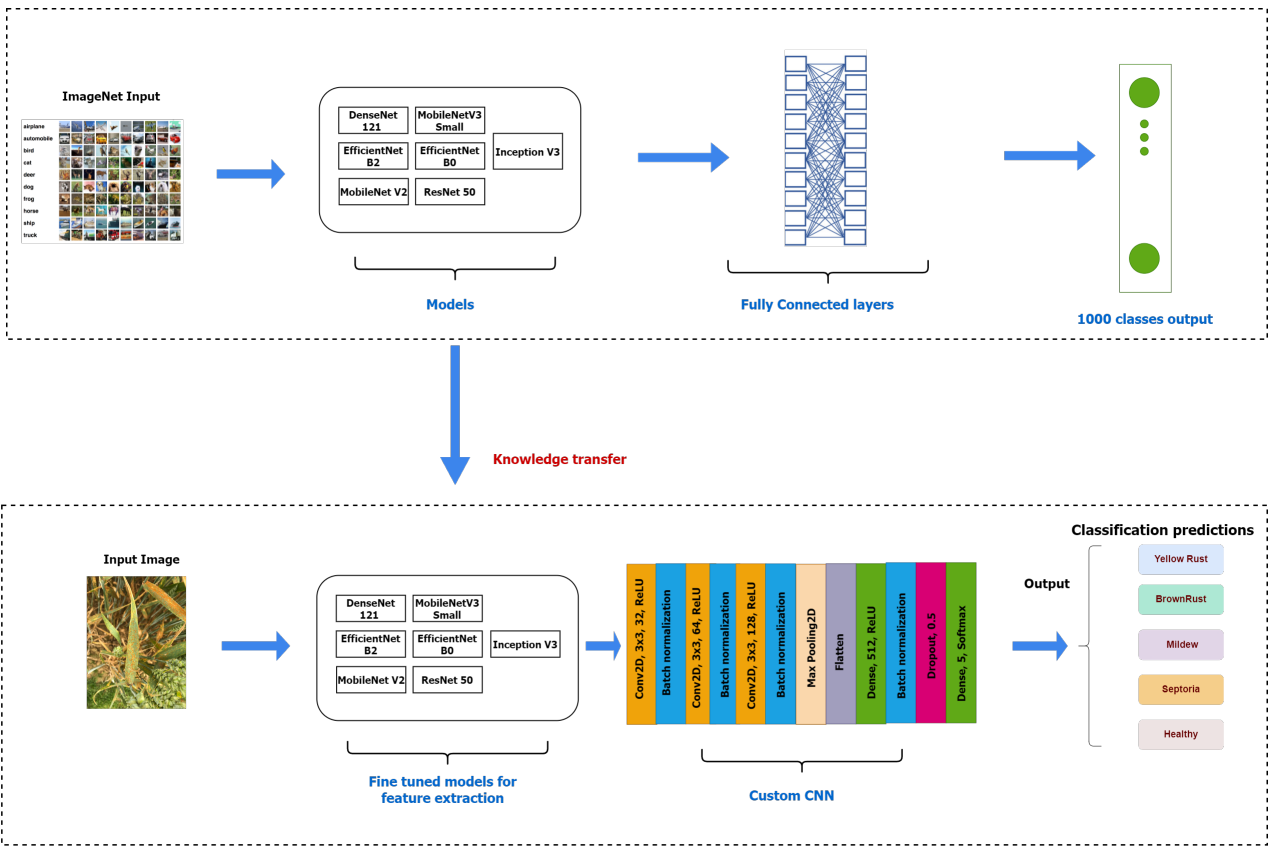
\includegraphics[width=0.8\textwidth]{chapters/chapter1/images/Figure15.png}
%     \caption{Integration of the custom \gls{abb:cnn} with transfer learning networks \parencite{jouini2024wheat}.}
%     \label{fig:figure15}
% \end{figure}

% Transfer learning is especially valuable in agriculture, where acquiring large annotated datasets is difficult. By leveraging pre-trained models, researchers and practitioners can build effective models for plant disease detection with limited data and reduced computational cost


% \subsection{Fine-Tuning Strategies for Agricultural Data}


% While basic fine-tuning involves unfreezing and retraining a subset of layers in a pretrained model, fine-tuning strategies can be further optimized when dealing with agricultural data, which often presents unique challenges such as class imbalance, limited samples, and high intra-class variability (e.g., similar symptoms across different plant diseases). 

% In this context, several fine-tuning strategies can be applied to improve model generalization and performance:
% \begin{itemize}
%     \item \textbf{Gradual Unfreezing:} Instead of unfreezing all layers at once, layers are incrementally unfrozen, starting from the top (fully connected layers) and moving backward. This helps prevent the model from losing previously learned useful features during early training stages \parencite{hossen2025transfer}.
%     \item \textbf{Discriminative Learning Rates:} Assigning different learning rates to different layers, lower for earlier layers and higher for later ones, ensures that the more generic features are preserved while higher-level representations are fine-tuned for the new task \parencite{hossen2025transfer}.
%     \item \textbf{Early Stopping and Regularization:} Due to limited data, it's essential to prevent overfitting during fine-tuning. Techniques like early stopping, dropout, and weight decay can help maintain model robustness \parencite{li2021implicit}.
%     \item \textbf{Data Augmentation and Balancing:} Supplementing fine-tuning with targeted data augmentation (e.g., rotation, brightness adjustments, zoom) helps the model generalize better. In addition, synthetic oversampling techniques like SMOTE can address class imbalance issues \parencite{aquino2017effect}.
% \end{itemize}

% These strategies, when integrated thoughtfully, allow researchers to tailor fine-tuning to the specific nature of agricultural datasets, maximizing the benefits of transfer learning even in data-constrained environments.


\subsection{Object detection}
In the context of precision agriculture, object detection has emerged as a critical computer vision technique for automating the assessment of crop health by enabling the identification and localization of diseases, nutrient deficiencies, and weeds, thereby supporting more efficient and timely interventions on a large scale.

At its core, object detection involves predicting both the category and precise location of objects within an image, thus combining classification with localization. Traditional approaches consist of stages such as region proposal, feature extraction, and object classification. Over time, detection methods have evolved to address increasing demands for accuracy and speed, giving rise to both two-stage and one-stage detection frameworks \parencite{zhao2019objectdetection}.

Here are more details about the concepts of object detection: 
\begin{itemize}
    \item \textbf{Informative Region Selection} focuses on identifying likely object areas in an image to reduce computation by avoiding full image scans. While early methods like sliding windows were costly and redundant, modern approaches use region proposal algorithms or attention mechanisms to efficiently target relevant areas, especially useful in agricultural images with variable object sizes and shapes.
    \item \textbf{Feature Extraction} is the process of isolating important visual attributes from an image to effectively represent objects. Traditional methods, such as Scale Invariant Feature Transform (SIFT), Histograms of Oriented Gradients (HOG), and Haar-like features were designed to mimic human vision by focusing on edges, textures, and patterns. However, these handcrafted techniques often faced difficulties in real-world conditions due to variations in object appearance, lighting, and cluttered backgrounds, limiting their reliability in complex environments.
    \item \textbf{Classification and Localization} refer to the process of both identifying the object in an image and determining its precise location through bounding boxes. With the rise of deep learning, this step underwent a significant transformation. Models such as R-\gls{abb:cnn} and its subsequent versions: Fast R-\gls{abb:cnn}, Faster R-\gls{abb:cnn}, and \gls{abb:yolo} automated the feature extraction process and seamlessly integrated classification with bounding box regression. These advancements led to substantial improvements in both detection accuracy and processing speed, enabling real-time applications in fields like crop monitoring and pest detection.
\end{itemize}

% \subsubsection{Annotation of objects}
% Annotation refers to the process of labeling the objects (such as pests, diseases, or damaged crops) in the images by drawing bounding boxes around them and assigning class labels. This is a critical step for supervised learning, where the model learns to identify patterns based on labeled data. Several annotation techniques can be used:
% \begin{itemize}
%     \item \textbf{Bounding Boxes:} The most common annotation method in object detection. Each object is enclosed in a rectangular box, and the class of the object is assigned to it (e.g., "rust", "aphid").
%     \item \textbf{Polygons:} For more precise object delineation, especially when objects have irregular shapes (e.g., plant leaves affected by disease), polygons are used instead of bounding boxes.
%     % \item \textbf{Semantic Segmentation:} In cases where the task involves classifying each pixel in the image, semantic segmentation labels each pixel to indicate which class it belongs to (e.g., diseased or healthy tissue in a leaf).
% \end{itemize}

\subsubsection{Evaluation metrics in object detection}    
In object detection, several metrics are used to assess model performance:
\begin{itemize}
    \item \textbf{Mean Average Precision (mAP):} Measures the average precision across all object classes, balancing precision and recall to evaluate overall model performance.
    \item \textbf{Intersection over Union (IoU):} Calculates the overlap between predicted and ground truth bounding boxes, indicating localization accuracy. Higher IoU means better localization.
    
    \item \textbf{Precision:} Measures the proportion of true positive detections out of all predicted objects.
    \item \textbf{Recall:} Measures the proportion of true positive detections out of all actual objects.
   
    \item \textbf{F1-Score:} The harmonic mean of precision and recall, providing a balance between both.
    \item \textbf{Average Recall (AR):} Evaluates recall at different IoU thresholds, useful for detecting small objects or handling occlusions.
    \item \textbf{Confusion Matrix:} Summarizes true positives, false positives, true negatives, and false negatives, providing insights into model errors.
    \item \textbf{Speed Metrics} like frames per second (FPS) and latency measure how fast an object detection model works in real time. FPS shows how many images the system can handle each second, higher FPS means smoother, faster image analysis. Latency is the time it takes to process one image and give a result, lower latency means quicker response.
    \item \textbf{AP at Specific IoU Thresholds:} Measures precision at different IoU levels to understand performance under stricter conditions.
\end{itemize}

\subsubsection{Key architectures}
Many architectures are designed to efficiently and accurately detect objects in images, even in complex agricultural environments. Below, we discuss four of the most widely used and effective object detection models: \gls{abb:yolo}, R-\gls{abb:cnn}, and \gls{abb:ssd}. 

\subsubsection{You Only Look Once (\gls{abb:yolo})}
\gls{abb:yolo} is a fast and efficient object detection framework that predicts both object confidences and bounding boxes (BBs) using the entire topmost feature map. The image is divided into a $S \times S$ grid, where each grid cell is responsible for predicting objects centered within it. Each cell predicts multiple bounding boxes and their corresponding confidence scores, which reflect the likelihood of an object being present and how well the predicted box overlaps with the ground truth (IoU) (see figure~\ref{fig:figure16}).

At test time, class-specific confidence scores are computed by multiplying the box confidence with conditional class probabilities. \gls{abb:yolo} optimizes a loss function during training to fine-tune predictions and improve detection accuracy \parencite{zhao2019objectdetection}.

\begin{figure}[H] % 'H' needs \usepackage{float}
    \centering
    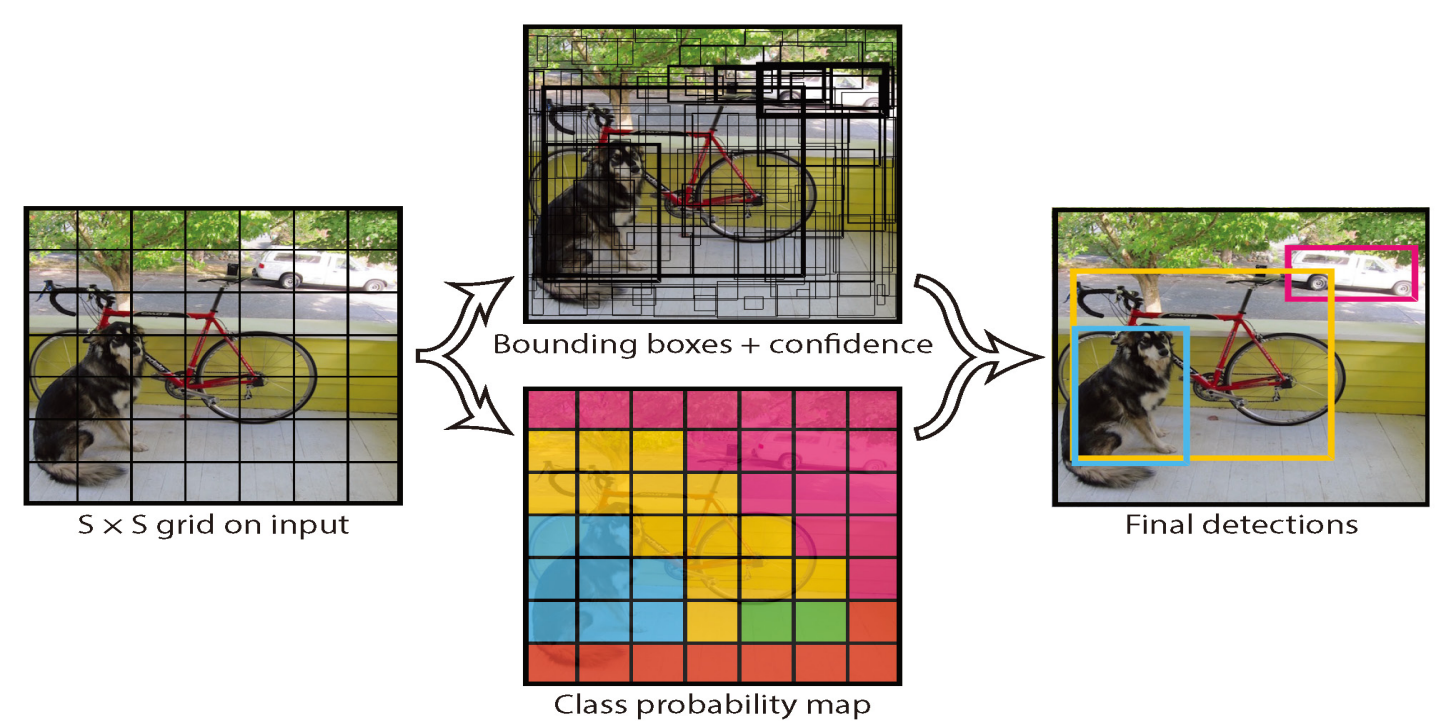
\includegraphics[width=0.8\textwidth]{chapters/chapter02/images/Figure16.png}
    \caption{Main idea of \gls{abb:yolo} \parencite{zhao2019objectdetection}.}
    \label{fig:figure16}
\end{figure}

\subsubsection{R-\gls{abb:cnn}}
R-\gls{abb:cnn} is a significant advancement in object detection, improving the quality of candidate bounding boxes (BBs) and utilizing deep architecture for high-level feature extraction \parencite{zhao2019objectdetection}. It consists of three main stages, as presented in figure~\ref{fig:figure17}:

\begin{itemize}
    \item \textbf{Region Proposal Generation:} R-\gls{abb:cnn} uses selective search to generate about 2000 region proposals per image, improving candidate box accuracy and reducing the search space.
    \item \textbf{\gls{abb:cnn}-Based Feature Extraction:} Each region proposal is resized and passed through a \gls{abb:cnn} to extract a 4096-dimensional feature, creating a high-level, robust representation of the object.
    \item \textbf{Classification and Localization:} Region proposals are classified using pre-trained linear SVMs, and bounding box regression is applied. Non-maximum suppression (NMS) is used to eliminate redundant boxes and finalize object detections.
\end{itemize}

\begin{figure}[H] % 'H' needs \usepackage{float}
    \centering
    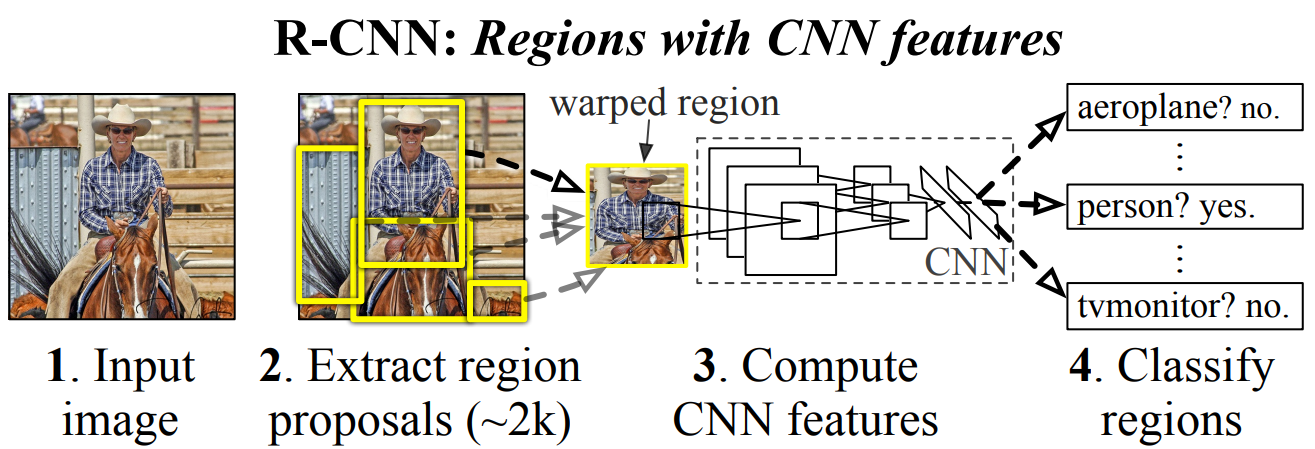
\includegraphics[width=0.9\textwidth]{chapters/chapter02/images/Figure17.png}
    \caption{Flowchart of R-\gls{abb:cnn} \parencite{zhao2019objectdetection}.}
    \label{fig:figure17}
\end{figure}

Despite its success, R-\gls{abb:cnn} has drawbacks, including slow inference due to \gls{abb:cnn} computation for each region, time-consuming multistage training, high memory and storage requirements for storing region features, and redundant region proposals from selective search that slow down the process \parencite{zhao2019objectdetection}.


% \paragraph{Faster R-\gls{abb:cnn}}


% Faster R-\gls{abb:cnn} improves upon earlier object detection models by introducing a Region Proposal Network (RPN), a deep learning-based method for generating object proposals, which shares convolutional features with the detection network to generate object proposals efficiently, eliminating the need for methods like selective search. The RPN uses a fully convolutional network (FCN) (as presented in Figure~\ref{fig:figure18}) to predict bounding boxes and object scores simultaneously. The system uses anchors of multiple scales and aspect ratios and is trained end-to-end with a multitask loss function. While Faster R-\gls{abb:cnn} achieves state-of-the-art accuracy and high-speed processing, it is limited by its alternate training algorithm, which is time-consuming and struggles with extreme object scales and shapes \parencite{zhao2019objectdetection}.

% \begin{figure}[H] % 'H' needs \usepackage{float}
%     \centering
%     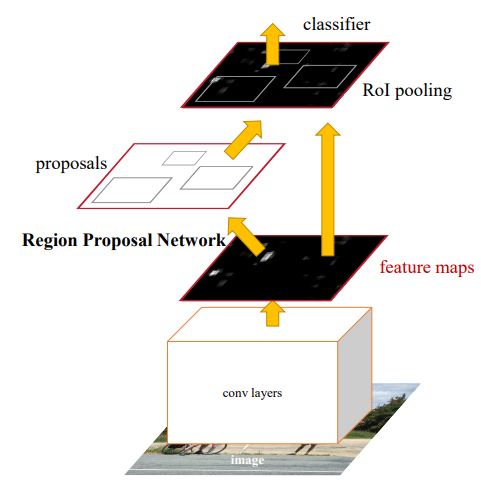
\includegraphics[width=0.6\textwidth]{chapters/chapter1/images/Figure18.png}
%     \caption{An illustration of the Faster R-\gls{abb:cnn} model \parencite{ren2016faster}.}
%     \label{fig:figure18}
% \end{figure}

\subsubsection{Single Shot Multibox Detector (\gls{abb:ssd})}
The \gls{abb:ssd} model was developed to overcome limitations in \gls{abb:yolo}, especially with small and irregularly shaped objects. Unlike YOLO’s fixed grid strategy, SSD utilizes multiple default anchor boxes of varying aspect ratios and scales, enabling better detection across object sizes. It combines predictions from multiple resolution feature maps and employs a VGG16 backbone with added layers for object localization and classification (see Appendix~\ref{app:annexA}). SSD uses a combination of localization and confidence loss during training and refines results using non-maximum suppression. It achieves higher accuracy than Faster R-CNN on PASCAL VOC and COCO, while being significantly faster at 59 fps for 300×300 input, though performance on small objects remains an area for improvement \parencite{zhao2019objectdetection}.

The architecture of \gls{abb:ssd} is illustrated in Figure~\ref{fig:figure19}, highlighting the VGG16 backbone, additional feature layers, and classifier convolutions.

\begin{figure}[H]
\centering
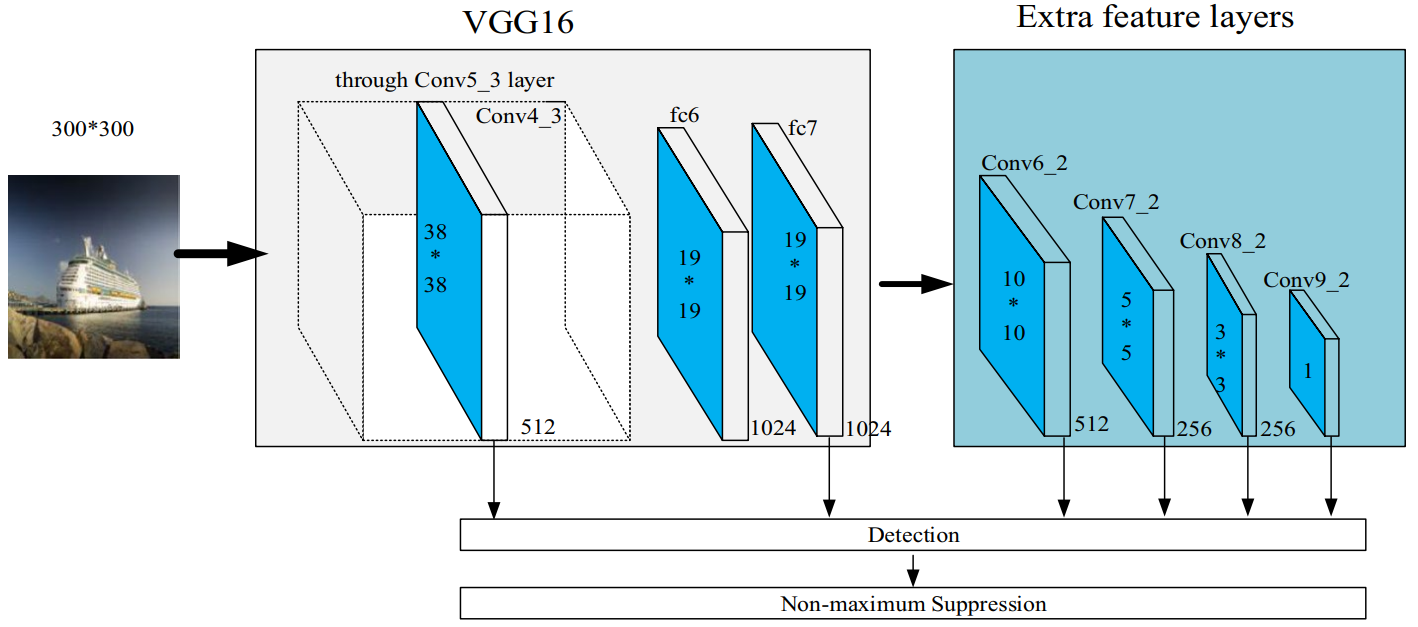
\includegraphics[width=0.9\textwidth]{chapters/chapter02/images/Figure19.png}
\caption{Architecture of \gls{abb:ssd} \parencite{li2021water}.}
\label{fig:figure19}
\end{figure}


\subsection{Image segmentation}
Image segmentation is a computer vision task that involves partitioning an image into multiple segments, or regions, to make the analysis of its content more manageable. Each pixel is classified into a specific category, which helps in identifying objects or boundaries within an image. In wheat disease detection, image segmentation is crucial for isolating affected areas and distinguishing between healthy and diseased plant tissues. Models like \gls{abb:pspnet}, U-Net and its variants, and DeepLabV3+ are particularly effective for this task, as they can capture both fine details and global context, leading to more accurate disease detection.

\subsubsection{Pyramid Scene Parsing Network (PSPNet)}
\gls{abb:pspnet} is a deep convolutional neural network architecture designed for semantic segmentation tasks, particularly effective in capturing both local and global contextual information. The core innovation of \gls{abb:pspnet} lies in its Pyramid Pooling Module (PPM), which aggregates context from different regions of the image at multiple scales. This is achieved by applying pooling operations at varying grid sizes, then upsampling and concatenating these pooled features with the original feature maps \parencite{pan2021deep}. This fusion allows \gls{abb:pspnet} to understand the spatial hierarchy and global structure of scenes more effectively than traditional \gls{abb:cnn}s (Figure~\ref{fig:PSPNet}). \gls{abb:resnet} and its variants are usually used as the backbone for \gls{abb:pspnet} due to their residual (skip) connections, which help alleviate the vanishing gradient problem and enable effective training of deep networks, making them well-suited for extracting rich feature representations in segmentation tasks.
\begin{figure}[H] % 'H' needs \usepackage{float}
    \centering
    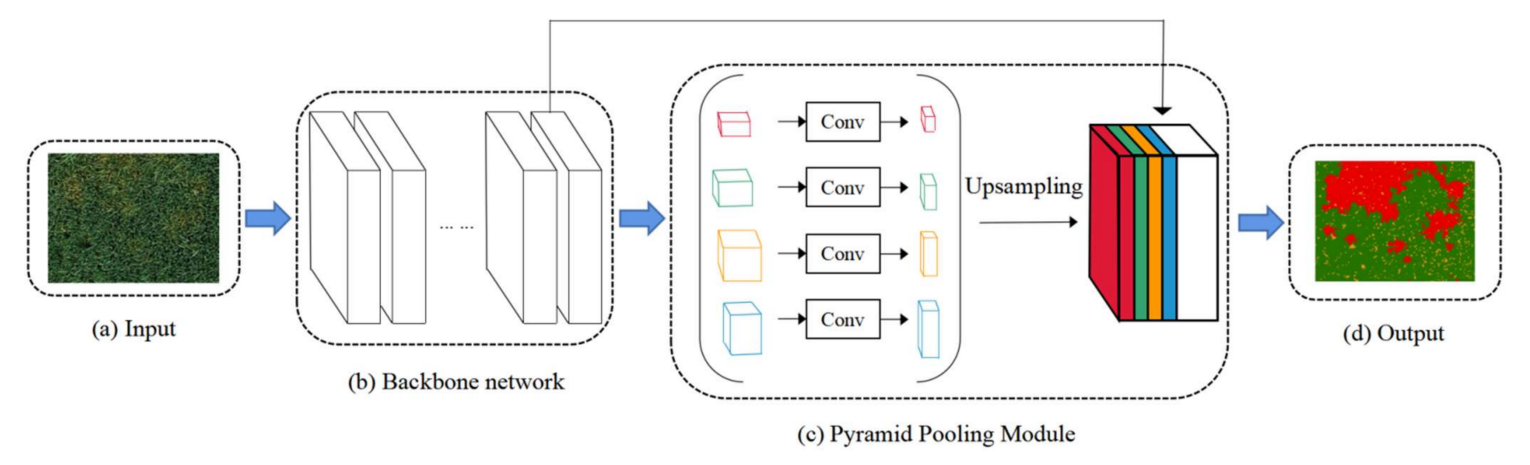
\includegraphics[width=0.9\textwidth]{chapters/chapter02/images/Figure20.png}
    \caption{Semantic Segmentation of Wheat Yellow Rust Using \gls{abb:pspnet} \parencite{pan2021deep}.}
    \label{fig:PSPNet}
\end{figure}

\subsubsection{U-Net model architecture}
U-Net is a convolutional neural network architecture designed for semantic segmentation, featuring a symmetric encoder-decoder structure. The encoder, or contracting path, captures contextual features using repeated 3×3 convolutions with ReLU activation, followed by 2×2 max pooling for downsampling. The decoder, or expansive path, performs upsampling and applies 3×3 convolutions to recover spatial resolution. Crucially, skip connections between corresponding encoder and decoder layers preserve high-resolution features, improving segmentation accuracy. A final 1×1 convolution maps the feature maps to the desired number of output classes. All convolutions use "same" padding with stride [1,1], and max pooling uses stride [2,2] with zero padding. ReLU activation is applied throughout the network, and input images undergo zero-center normalization for training stability \parencite{su2020aerial}. This architectural layout, including feature map sizes and layer depths, is depicted in Figure~\ref{fig:U-Net}.
\begin{figure}[H] % 'H' needs \usepackage{float}
    \centering
    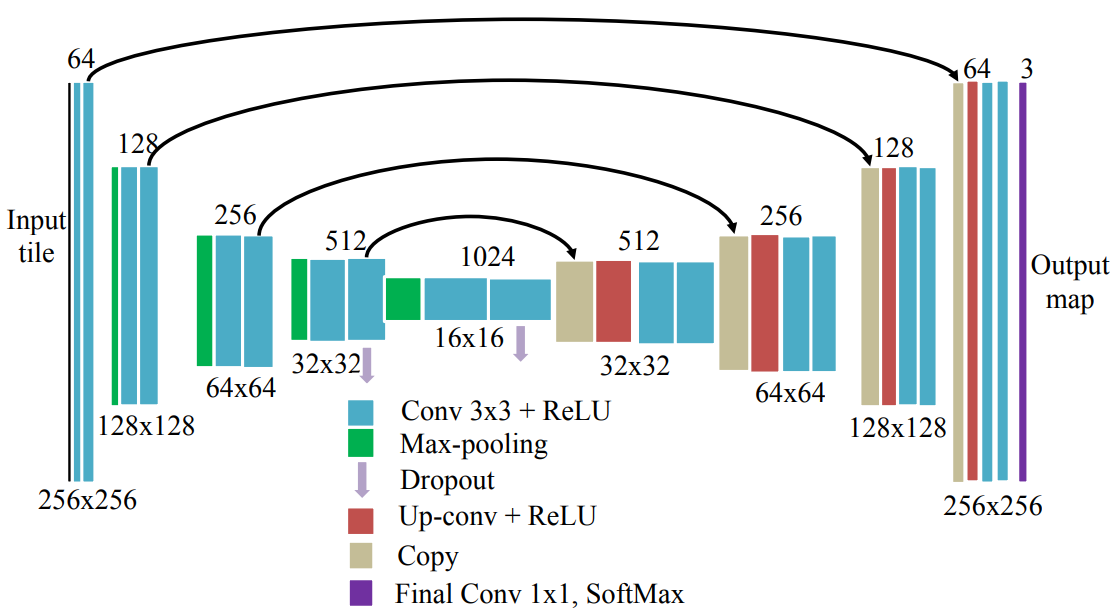
\includegraphics[width=0.8\textwidth]{chapters/chapter02/images/Figure21.png}
    \caption{U-Net Architecture for Semantic Segmentation \parencite{su2020aerial}.}
    \label{fig:U-Net}
\end{figure}
Several U-Net variants have been proposed to address computational efficiency and feature enhancement:
\begin{itemize}
    \item \textbf{LR-UNet (Lightweight Residual U-Net)}: This architecture introduces residual connections and lightweight convolutional blocks to reduce the number of parameters and computational cost while maintaining segmentation performance. It is especially suitable for deployment in resource-constrained environments such as mobile or embedded devices \parencite{zhang2021irunet}.
    
    \item \textbf{DF-UNet (Dual Feature U-Net)}: This model enhances the original U-Net by fusing both shallow (low-level spatial) and deep (high-level semantic) features. This dual feature strategy improves the network's ability to detect fine edges and preserve structural details, particularly in complex segmentation tasks such as medical or remote sensing imagery. DF-UNet may also integrate attention mechanisms and refined skip connections for more effective feature reuse \parencite{zhang2022wheat}.
\end{itemize}

\subsubsection{DeepLabV3+}
DeepLabV3+ is an advanced semantic segmentation model that builds upon DeepLabV3 by combining powerful contextual feature extraction with precise boundary recovery. DeepLabV3 uses Atrous Spatial Pyramid Pooling (ASPP) to capture multi-scale contextual information through parallel atrous (dilated) convolutions with varying rates, allowing the model to extract rich semantic features without reducing spatial resolution too much. However, DeepLabV3 lacks a decoder and relies on simple bilinear upsampling, which limits its ability to recover fine object boundaries. DeepLabV3+ (Figure~\ref{fig:DeepLabv3+}) addresses this by introducing a decoder module that refines segmentation results, especially along object edges, by upsampling the encoder’s output and combining it with low-level features from earlier layers of the network, followed by a few convolutions for detail refinement. Additionally, DeepLabV3+ applies depthwise separable (atrous separable) convolutions in both the ASPP and decoder modules to reduce computational cost while maintaining high accuracy, resulting in a more accurate and efficient architecture \parencite{chen2018encoder}.
\begin{figure}[H] % 'H' needs \usepackage{float}
    \centering
    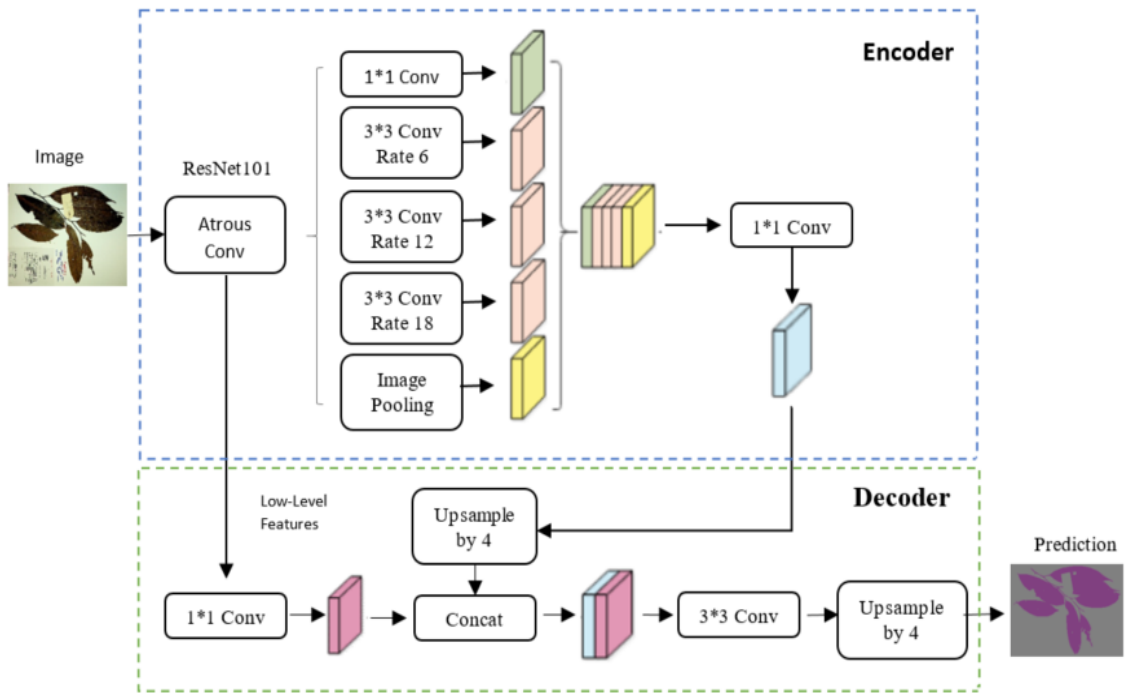
\includegraphics[width=0.9\textwidth]{chapters/chapter02/images/Figure22.png}
    \caption{DeepLabv3+ architecture \parencite{hussein2020semantic}.}
    \label{fig:DeepLabv3+}
\end{figure}

% \section{Challenges of Deep Learning in Agricultural Contexts}

% Despite the promising performance of deep learning and object detection in various fields, their application in agriculture presents a range of specific challenges. One of the primary issues is the limited availability of large, annotated agricultural datasets, which hampers the training of robust and generalizable models. Unlike natural image datasets like ImageNet, agricultural datasets often suffer from class imbalance, incomplete labeling, and domain specificity (e.g., crop types, diseases, and environmental conditions) \parencite{alzubaidi2021review}.

% Another challenge is the high intra-class variability and low inter-class variability found in agricultural images. For instance, symptoms of different diseases may look visually similar, or the same disease may appear differently across plant species and growth stages. Additionally, variations in lighting, occlusion by leaves, overlapping plants, and background clutter significantly affect detection performance \parencite{alzubaidi2021review}.

% The seasonal and geographic diversity further complicates the generalization of models trained on limited datasets. Moreover, the deployment of deep learning models in real agricultural environments must consider limited computing resources, especially for edge or mobile devices used in fields.

% Lastly, ensuring the interpretability and trustworthiness of AI decisions is crucial in agricultural contexts, as these technologies directly impact yield, resource use, and farmers’ livelihoods. Addressing these challenges requires collaborative efforts in data collection, annotation, model adaptation, and efficient deployment strategies \parencite{alzubaidi2021review}.

% \section{Challenges of Deep Learning in Agricultural Contexts}

% While deep learning has shown strong performance across various domains, its application in agriculture faces unique challenges. Limited and imbalanced annotated datasets, high intra-class variability, and low inter-class variability hinder model generalization. Factors such as lighting changes, leaf occlusion, and cluttered backgrounds further reduce detection accuracy \parencite{alzubaidi2021review}. Moreover, most models rely on close-range imagery, which restricts early-stage detection over large fields. Integrating remote sensing (e.g., hyperspectral or multispectral imaging) with deep learning helps address these limitations by enabling large-scale monitoring and identifying stress indicators before symptoms appear. This fusion significantly improves accuracy and supports scalable, cost-effective disease management \parencite{wang2024integration}.

\section{Conclusion}
In this chapter, we explored key deep learning concepts and models used for image-based recognition tasks, focusing on classification, object detection, and semantic segmentation. These techniques are essential for automating and improving agricultural workflows, especially in crop health monitoring. Building on this foundation, The next chapter explores how these techniques can be integrated with remote sensing data for early and accurate detection of wheat diseases.









% Enhancing Wheat Disease Detection: Why Remote Sensing is Crucial Beyond ML/DL Alone

% While machine learning (ML) and deep learning (DL) have revolutionized plant disease detection through their ability to automatically learn patterns from data, relying on these methods alone for wheat disease detection reveals several critical limitations. First, ML/DL models require large volumes of high-quality labeled images to perform well—collecting and annotating such datasets in agricultural environments is labor-intensive, costly, and often impractical. Second, most existing ML/DL systems depend on close-range images taken with smartphones or hand-held devices, limiting their ability to detect early-stage diseases that manifest at a larger field scale. Third, these models are highly sensitive to environmental variations such as lighting conditions, leaf occlusion, and weather changes, which can lead to poor generalization and reduced accuracy in real-world scenarios. Remote sensing (RS) technologies provide a powerful solution to these challenges. By capturing hyperspectral or multispectral data (e.g., NDVI indices), RS can identify subtle stress indicators in wheat crops before visual symptoms appear. Additionally, satellite and UAV platforms offer large-scale, continuous field monitoring that’s not feasible with ground-based imagery alone. When RS data is fused with ML/DL models, it significantly enhances disease classification performance—studies show improvements exceeding 20% in accuracy. Thus, integrating remote sensing with AI techniques is not just beneficial but essential for overcoming limitations in data availability, environmental variability, and scalability, ultimately enabling more accurate, timely, and cost-effective wheat disease management at both the local and regional levels \parencite{wang2024integration}.